\section{Motivation}
\label{sec:motivation}

In this section, we motivate our ideas via an example written in
\txnimp - a functional language equipped with a \C{DB} monad to
compose database computations. Besides the usual \C{bind} and
\C{return} combinators, monad offers a \C{txn\_do} combinator that
executes a database computation and returns the result. 

\begin{figure}
\centering
\begin{ocaml}
let new_order_txn d_id c_d_id c_id
      (ireqs: item_req list) = atomically do
  dist <- SQL.select1 District (fun d -> d.d_id = d_id);
  let o_id = dist.d_next_o_id;
  SQL.update District (fun d -> {d with d_next_o_id =d_next_o_id + 1})
                      (fun d -> d.d_id = d_id );
  SQL.insert Order {o_id=o_id;  o_d_id=d_id; 
                    o_c_id=c_id; o_ol_cnt=S.size ireqs; };
  SQL.insert New_order {no_o_id=o_id; no_d_id=d_id};
  foreach ireqs @@ fun ireq -> do
    stk <- SQL.select1 Stock (fun s -> s.s_i_id = ireq.ol_i_id);
    let s_qty' = if stk.s_qty >= ireq.ol_qty + 10 
                then stk.s_qty - ireq.ol_qty 
                else stk.s_qty - ireq.ol_qty + 91;
    SQL.update Stock (fun s -> {s with s_qty = s_qty'}) 
                     (fun s -> s.s_i_id = ireq.ol_i_id);
    SQL.insert Order_line {ol_o_id=o_id; ol_d_id=d_id; 
                           ol_i_id=ireq.ol_i_id; ol_qty=ireq.ol_qty}
 
\end{ocaml}
\caption{\small Concurrent withdraw transactions}
\label{fig:motiv-eg-1}
\vspace*{-10pt}
\end{figure}

Consider an implementation of a banking application that admits
concurrent withdraw transactions on an account balance (\C{B}), as
shown in Fig.~\ref{fig:motiv-eg-1}. If the initial balance (\C{k}) in
the account is enough to perform both withdraws, then the final
balance, after both transactions commit, is expected to reflect the
effects of both withdraws. The pre- and post-conditions in
Fig.~\ref{fig:motiv-eg-1} reflect this expectation. Indeed, invariants
are guaranteed to hold if both withdraw transactions are serialized,
making \iso{Serializable} isolation ({\sc ser}) level a sufficient
condition to preserve invariants. But, is {\sc ser} necessary?

As an alternative, consider the execution of this transaction under a
\emph{Read Committed} ({\sc rc}) isolation level, which is weaker than
{\sc ser}.\footnote{{\sc rc} is in fact the default isolation level in
Postgres 9.5 and Oracle 11g databases.} An {\sc rc} transaction is
isolated from the writes of uncommitted transactions, and is therefore
free from \emph{dirty reads}~\cite{berenson} of uncommitted data. In
the current example, {\sc rc} isolation admits the two executions
shown in Fig.~\ref{fig:rc-ex} on a strongly consistent ({\sc sc})
store, such as a conventional RDBMS.

\begin{figure}[!h]
\centering
\subcaptionbox {
  {\sc rc} Execution 1
  \label{fig:motiv-eg-1-a}
} [
  0.55\columnwidth
] {
  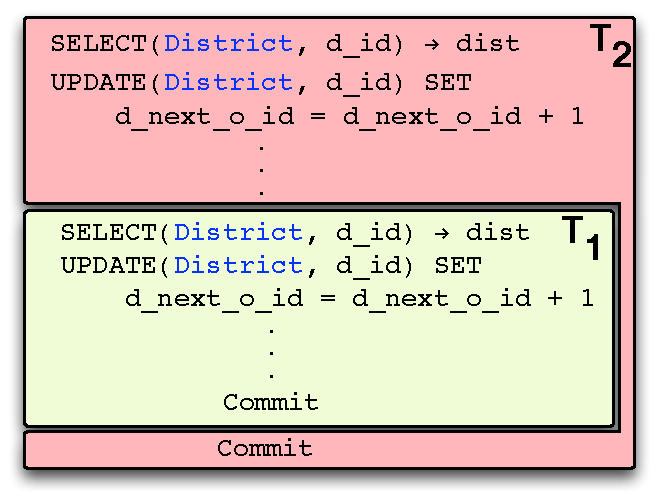
\includegraphics[scale=0.6]{Figures/motiv-eg-1-a}
}
%\hspace*{0.5in}
\subcaptionbox {
  {\sc rc} Execution 2
  \label{fig:motiv-eg-1-b}
}{
  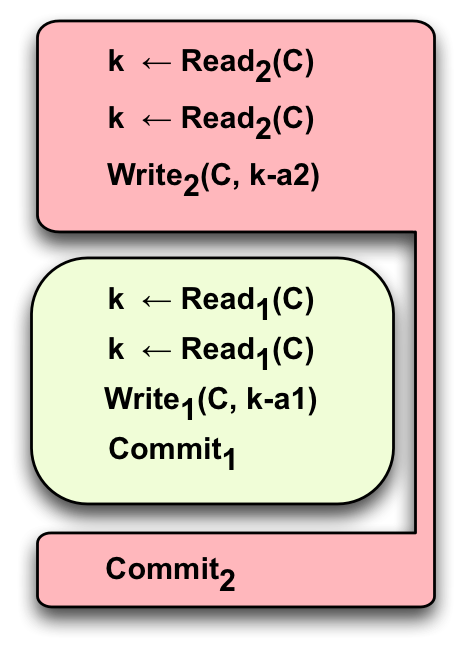
\includegraphics[scale=0.6]{Figures/motiv-eg-1-b}
}
\caption{\small A possible execution of the program shown in Fig.~\ref{fig:motiv-eg-1} under
  \iso{Read Committed} isolation level. Transaction \C{Wd1} is shown
  against lighter green background, and transaction \C{Wd2} against
  darker red background. Each transaction reads the balance (\C{B})
  twice, hence two \C{Reads}.}
\label{fig:rc-ex}
\end{figure}

The figure depicts an execution as a series of read, write, and commit
operations. In the execution on left, transaction \C{Wd1} (green)
reads the current balance (\C{k}) and writes the new balance
(\C{k-a1}), but before it commits, transaction \C{Wd2} (red) executes
and commits, writing the new balance (\C{k-a2}). {\sc rc} isolation
prevent \C{Wd2} from witnessing the uncommitted writes of transaction
\C{Wd1}.  Subsequently committing \C{Wd1} leads to the loss of
\C{Wd2}'s updates (the so-called \emph{lost update
anomaly}~\cite{berenson}), resulting in an incorrect balance of
\C{k-a1}. The execution on right describes a similar scenario with
\C{Wd1} and \C{Wd2} exchanging their roles.  Clearly, {\sc rc} is an
excessively weak isolation level for this program because it loses the
updates of one transaction, resulting in the violation of the
post-condition.  A stronger isolation level that prevents lost updates
is required. \iso{Snapshot Isolation} ({\sc si})~\cite{berenson} fits
this requirement; {\sc si} effectively serializes transactions that
update a shared data object by aborting and re-executing a transaction
if write-write conflicts are detected during its commit.\footnote{{\sc
si} however does not serialize transactions in the absence of
write-write conflicts.} Since {\sc si}, unlike {\sc ser}, does not
need expensive mechanisms such as lock-based concurrency control or
runtime monitoring, it is also more efficient, making it appropriate
for both withdraw transactions.

Thinking in terms of anomalies, as described above, is how database
programmers are often encouraged to reason about weak isolation.
Unfortunately, such reasoning does not rest on any sound foundation,
and is thus highly error-prone. Reasoning in terms of how weak
isolation variants are implemented is no better since it requires
programmers to understand low-level implementation details of the
database that are far removed from the application semantics. An
attractive  alternative in this context would be a principled
reasoning approach that combines declarative reasoning about isolation
guarantees with operational reasoning about programs. We demonstrate
how our proof system makes this possible in the context of the current
example.

First, we note that the example in Fig.~\ref{fig:motiv-eg-1} is a
concurrent program, and hence is amenable to \emph{rely-guarantee}
style reasoning~\cite{rgjones}, a compositional proof technique that
allows us to reason about the behaviour of individual threads by
abstracting away interferences induced by other threads (collectively
called \emph{the environment}) into a \emph{rely} relation. In an
ordinary concurrent program, every environment step is a valid
interference in the current thread. However, in the presence of
transactions executing under various levels of weak isolation,
determining what constitutes an interference is a non-trivial problem.
For example, a \iso{Serializable} transaction admits no interference,
whereas within a transaction executing under \iso{Read Uncommitted}
isolation, all interferences are valid. Between these two extremes are
various levels of isolation that admit some interferences while
prohibiting others. For example, \iso{Read Committed} isolation admits
interference of a committed transaction, but not those from
uncommitted transactions. \iso{Snapshot Isolation} admits interference
from committed non-conflicting transactions, and so on.

\begin{figure}
\begin{smathpar}
\begin{array}{lcl}
\psi_{RC} & \defeq & \forall T_1,T_2,\eta_1,\eta_2.\; \txn(\eta_1) = T_1 
  \conj \txn(\eta_2) = T_2 \\
  & & \hspace*{0.6in}\conj T_1 \neq T_2 \conj \eta_1 \hboar
  \eta_2 \Rightarrow T_1 \hboar \eta_2 \\
\psi_{SI} & \defeq & \forall T_1,T_2.\; T_1 \neq T_2 \conj
  (\exists \C{X}.~{T_1 \wrstoar \C{X}} \conj 
                      {T_2 \wrstoar \C{X}})\\
  &  & \hspace*{0.6in}\Rightarrow{T_1 \hboar T_2} \disj {T_2 \hboar T_1} \\
\end{array}
\end{smathpar}
\caption{\small Interference properties for different weak isolation
levels can be captured as constraints over the happens-before
relation.}
\label{fig:interference-ex}
\end{figure}

\begin{figure}
\centering
\subcaptionbox {
  \label{fig:hb-eg-1}
} [
  0.25\columnwidth
] {
  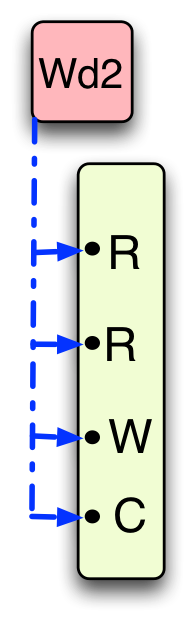
\includegraphics[scale=0.45]{Figures/hb-eg-1}
}
\subcaptionbox {
  \label{fig:hb-eg-2}
} [
  0.25\columnwidth
] {
  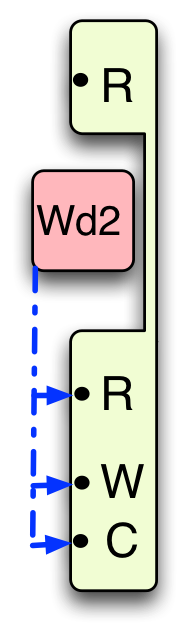
\includegraphics[scale=0.45]{Figures/hb-eg-2}
}
\subcaptionbox {
  \label{fig:hb-eg-3}
} [
  0.25\columnwidth
] {
  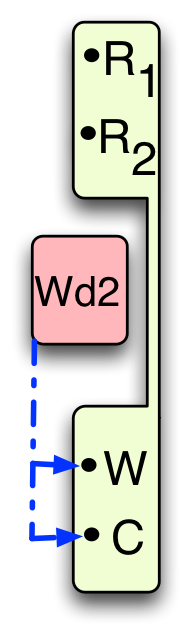
\includegraphics[scale=0.45]{Figures/hb-eg-3}
}
\subcaptionbox {
  \label{fig:hb-eg-4}
}{
  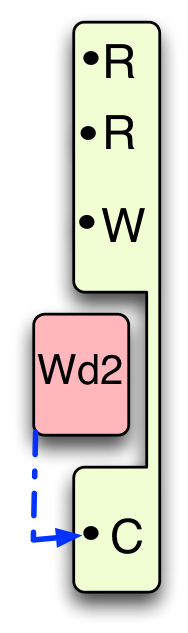
\includegraphics[scale=0.45]{Figures/hb-eg-4}
}


\caption{\small Possible executions for the example in
Fig.~\ref{fig:motiv-eg-1}. Letters R, W and C stand for read, write
and commit, respectively. Each blue dashed arrow represents a $\hbZ$
relationship between all operations of \C{Wd2} and an operation in
\C{Wd1}. $\psi_{SI}$ specification allows $\hbZ$ arrows (hence the
execution) in Fig.~\ref{fig:hb-eg-1}. $\psi_{RC}$ specification allows
$\hbZ$ arrows in
Figs.~\ref{fig:hb-eg-1},~\ref{fig:hb-eg-2},~\ref{fig:hb-eg-3}, and
~\ref{fig:hb-eg-4}.  }
\label{fig:motiv-eg-1-hb}
\vspace*{-8pt}
\end{figure}

For the rely-guarantee approach to be useful, it has to thus constrain
allowed interference in accordance with the chosen level of isolation
associated with a transaction. The first observation we make is that
we can constrain interference by constraining the nature of the
\emph{happens-before} ($\hbZ$) relation, which ultimately dictates
what other transactions become visible to a transaction, or its
constituents, and when. To do so, we axiomatize the $\hbZ$ relation to
capture the interference characteristics of different isolation levels
as their specifications. Two such specifications are
shown\footnote{Note that specifications presented here are solely for
illustration. The actual specifications described in
\S\ref{sec:ansi-isolation} are more nuanced.} in
Fig.~\ref{fig:interference-ex}. The \iso{Read Committed} specification
($\psi_{RC}$) allows an operation $\eta_1$ of a transaction $T_1$ to
happen-before an operation $\eta_2$ of another transaction $T_2$ only
if every operation in $T_1$ (including its commit) happens-before
$\eta_2$ (we let $T_1 \hboar \eta_2$ denote this). The specification
does not require $T_1$ to execute and commit before all operations of
$T_2$, thus allowing it to interfere in $T_2$, just as \C{Wd2}
interferes in \C{Wd1} in Fig.~\ref{fig:motiv-eg-1-a}. The
\iso{Snapshot Isolation} specification ($\psi_{SI}$) requires two
transactions that write to the same variable (denoted $\wrstoar$) to be
related by happens-before.  This effectively prohibits interference
due to actions in $T_1$ being interleaved in $T_2$ (or, vice versa). 

Fig.~\ref{fig:motiv-eg-1-hb} is a visualization of $\hbZ$ from \C{Wd2}
to \C{Wd1} allowed by $\psi_{RC}$ and $\psi_{SI}$. Arrows in all
executions are legal under $\psi_{RC}$ because in no execution does an
operation from \C{Wd2} happen-before an operation of \C{Wd1} without
the commit of \C{Wd2} also happening before the operation of \C{Wd1}.
$\psi_{SI}$ however disallows $\hbZ$ arrows (hence executions) in
Figs.~\ref{fig:hb-eg-2},~\ref{fig:hb-eg-3}, and~\ref{fig:hb-eg-4}
because such arrows establish $\hbZ$ edges between (operations in)
\C{Wd2} and only a subset of the operations in \C{Wd1}. Since the
result of an operation (\eg a read) depends on what happens before
that operation, the structure of the $\hbZ$ relation ultimately
dictates the final result of the program. The arrows in
Figs.~\ref{fig:hb-eg-1} and~\ref{fig:hb-eg-2} denote $\hbZ$
relationships that do not affect the value of \C{B} in a way that
causes the program to violate its post-condition. In contrast, arrows
in Figs.~\ref{fig:hb-eg-3} and~\ref{fig:hb-eg-4} denote $\hbZ$
relationships that lead to the violation of the post-condition. The
task of the reasoning framework is to determine if \emph{all} $\hbZ$
relationships allowed by an isolation level lead to the satisfaction
of the post-condition.

% There is a $\hb$ edge (first dashed) that is allowed by RC but
% prohibited by SI, which nonetheless does not lead to invariant
% violation. 

The specification of an isolation level encodes its interference
characteristics as constraints over the $\hbZ$ relation. However, for
this to be useful in reasoning about programs, the rely-guarantee
framework should be able to use the specification to determine if an
interference is valid or not, allowing the programmer to only focus on
valid interferences. Our second observation is that this is possible
if the reasoning framework adequately tracks $\hbZ$ at each program
point, while preserving $\hbZ$ constraints as invariants between
program points. An interference that leads to the violation of $\hbZ$
constraints (i.e., an invalid interference) is thus automatically
prohibited. For instance, consider the program point after the write
to \C{B} in \C{Wd1}. The expected invariant ($\phi$) at that program
point is shown below ($\committed$ stands for ``committed''):

\begin{smathpar}
\begin{array}{c}
 \neg\committed(\C{Wd1}) \conj \C{Wd1} \wrstoar \C{B}  \conj 
    (\neg\committed(\C{Wd2}) \Rightarrow \C{B = k-a1}) \\
    \conj (\committed(\C{Wd2})
                \Rightarrow \C{B = k-a1-a2})
\end{array}
\end{smathpar}

\noindent $\phi$ asserts that \C{Wd1} is not yet committed, and that
it wrote to \C{B}, and the value of \C{B} is either \C{k-a1-a2} or
\C{k-a1} depending on whether or not \C{Wd2} is committed. If $\phi$
remains invariant until \C{Wd1} commits, then the post-condition (\C{B
= k-a1-a2}) can be established easily. However, an interference from
\C{Wd2} at this stage (captured by the last dashed arrow in
Fig.~\ref{fig:motiv-eg-1-hb}) may violate the invariant by writing
$\C{k-a2}$ to \C{B} and committing \C{Wd2}, thus leading to
$\committed(\C{Wd2}) \Rightarrow \C{B=k-a2}$. Fortunately,
\iso{Snapshot Isolation} prevents this interference, and this can be
shown by demonstrating that an interference from \C{Wd2} starting from
an execution state that satisfies $\psi_{SI} \wedge \phi$ leads to an
execution state where neither $\C{Wd2} \hboar \C{Wd1}$ nor $\C{Wd1}
\hboar \C{Wd2}$ holds; $\C{Wd2} \hboar \C{Wd1}$ does not hold because
\C{Wd1}'s write to \C{B} clearly happened before \C{Wd2}'s commit, and
$\C{Wd1} \hboar \C{Wd2}$ does not hold because \C{Wd1} has not yet
committed, while \C{Wd2} has already begun. Since \C{Wd2} also writes
to \C{B}, this violates the $\psi_{SI}$ constraint which we assume to
be an invariant. A proof that the post-condition holds now follows
from the contradiction. It is informative to note that if the
invariant is $\psi_{RC}$ instead of $\psi_{SI}$, we cannot derive a
contradiction and we cannot rule out the interference, which
(rightfully) causes  the proof to fail.

Implicit in the above discussion is the assumption of a strongly
consistent ({\sc sc}) store that guarantees the visibility of all
previously committed transactions. An {\sc sc} semantics can be built
into the reasoning framework, leading to a proof system tailor-made
for such stores.  However, for the reasoning framework to be truly
useful, it should be capable of handling different consistency
semantics, supporting stores that are weaker than {\sc sc} (e.g.,
causally or eventually consistent), and should be able to reconcile
conflicts between consistency and isolation constraints.  We
demonstrate how our reasoning framework makes this possible in the
following sections.

%% We have thus far assumed a strongly consistent ({\sc sc}) store that,
%% in the absence of transactions with special isolation requirements,
%% makes the effects of any operation immediately visible to all
%% subsequent operations. The natural behaviour of {\sc sc} to totally
%% order all operations w.r.t. the $\hbZ$ relation could be in conflict
%% with the constraints imposed by weak isolation. To meet the
%% requirements of weaker isolation levels, say {\sc rc}, the store has
%% to adapt itself to \emph{hide} the effects of concurrent transactions
%% until they are committed. Once committed though, effects need to be
%% immediately visible to subsequent operations. This semantics can be
%% built into the reasoning framework, leading to a proof system
%% tailor-made for such stores. However, for the reasoning framework to
%% be truly useful, it has to be parametric over different consistency
%% semantics, supporting stores that are weaker than {\sc sc} (e.g.,
%% causally or eventually consistent), and should be able to reconcile
%% conflicts between consistency and isolation constraints.  We
%% demonstrate how our reasoning framework makes this possible in the
%% following sections.
